
\documentclass{article}
\usepackage[utf8]{inputenc}
\usepackage{graphicx}
\usepackage{subcaption}
\usepackage{tikz} 
 \usetikzlibrary{arrows,automata,positioning,petri}
 
\title{Report on Labwork 9}
\author{TRAN Thi Hong Hanh}

\begin{document}

\maketitle
\section{Explain how you implement the labwork?}
\begin{itemize}
    \item Implement Kuwahara filter following the instruction on the slide.
    \begin{verbatim}
__global__ void kuwahara(uchar3 *input, uchar3 *output, 
                            int width, int height, int winSize)
{
    int tidX = threadIdx.x + blockIdx.x * blockDim.x;
    if (tidX >= width)
        return;
    int tidY = threadIdx.y + blockIdx.y * blockDim.y;
    if (tidY >= height)
        return;
    int tid = tidY * width + tidX;

    double window[4] = {0.0};
    double SD[4] = {0.0};
    int meanRGB[4][3] = {0};
    int pxCount[4] = {0};
    int winPos;

    for (int x = 1 - winSize; x <= winSize - 1; x++)
    {
        for (int y = 1 - winSize; y <= winSize - 1; y++)
        {
            int rows = tidX + x;
            int columns = tidY + y;
            if (rows < 0 || rows >= width || columns < 0 || columns >= height)
                continue;
            int positionOut = rows + columns * width;

            int red = input[positionOut].x;
            int green = input[positionOut].y;
            int blue = input[positionOut].z;

            if (x >= 0 && y <= 0)
            {
                winPos = 3; // bottom right
            }

            if (x <= 0 && y <= 0)
            {
                winPos = 2; // bottom left
            }

            if (x >= 0 && y >= 0)
            {
                winPos = 1; //top right
            }

            if (x <= 0 && y >= 0)
            {
                winPos = 0; // top left
            }
            meanRGB[winPos][0] += red;
            meanRGB[winPos][1] += green;
            meanRGB[winPos][2] += blue;

            window[winPos] += max(red, max(green, blue));
            pxCount[winPos]++;

            SD[winPos] += pow((max(red, max(green, blue)) - window[winPos]), 2.0);
        }
    }

    for (int i = 0; i < 4; i++)
    {
        SD[i] = sqrt(SD[i] / (pxCount[i]));
        window[i] /= pxCount[i];
        for (int j = 0; j < 3; j++)
        {
            meanRGB[i][j] /= pxCount[i];
        }
    }

    double minSD = min(SD[0], min(SD[1], min(SD[2], SD[3])));
    if (minSD == SD[0])
        tidX = 0;
    else if (minSD == SD[1])
        tidX = 1;
    else if (minSD == SD[2])
        tidX = 2;
    else
        tidX = 3;

    output[tid].x = meanRGB[tidX][0];
    output[tid].y = meanRGB[tidX][1];
    output[tid].z = meanRGB[tidX][2];
}
    \end{verbatim}
    
    \item Command:
    \begin{verbatim}
        ./labwork 10 ../data/cloud.jpeg 
    \end{verbatim}
    \item Result:
    \begin{verbatim}
    USTH ICT Master 2019, Advanced Programming for HPC.
    Warming up...
    Starting labwork 10
    [ALGO ONLY] labwork 10 ellapsed 513.5ms
    Labwork 10 ellapsed 520.9ms
    \end{verbatim}
    \begin{figure}[h]
      \centering
      \begin{subfigure}{.45\textwidth}
        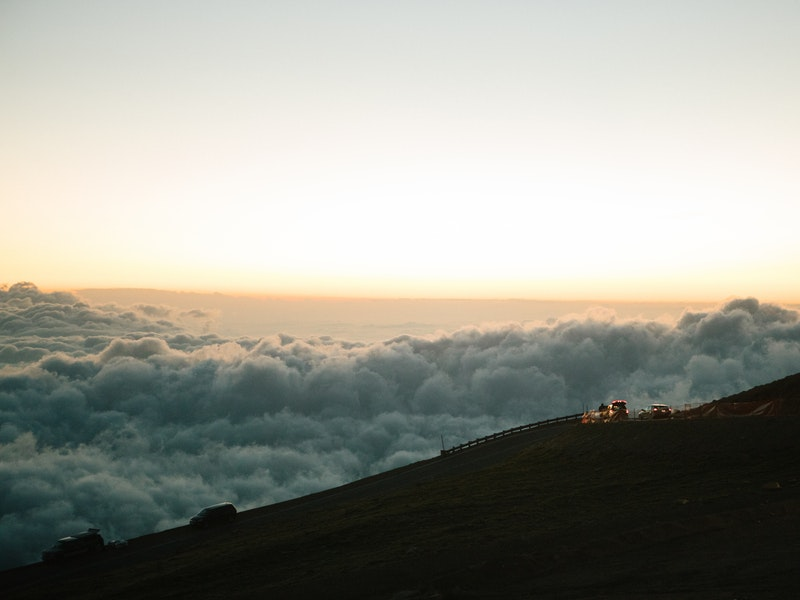
\includegraphics[width=\linewidth]{./result/cloud.jpeg}
        \caption{Original image}
      \end{subfigure}
      \hspace{1cm}
      \begin{subfigure}{.45\textwidth}
        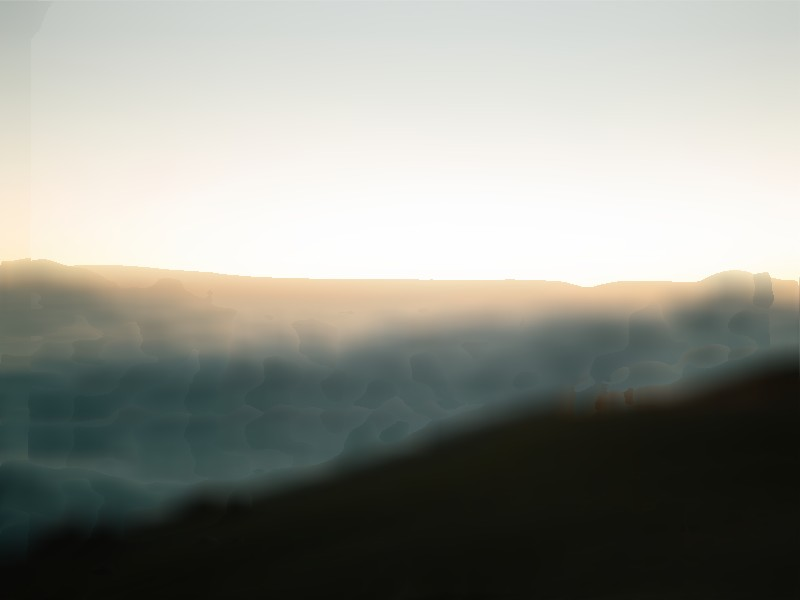
\includegraphics[width=\linewidth]{./result/labwork10-gpu-out.jpg}
        \caption{Fine-art transformation}
      \end{subfigure}
    \caption{The output image after fine-art transformation compared to the original one.}
    \end{figure}
\end{itemize}


\end{document}

